Ben Trout

2014-10-31

Building Intake, CAD

\begin{tabular}{|p{5cm}|p{5cm}|}
\hline
 Building Intake&
Nick and I with the help of some other team members were in charge of starting the robot. While I worked on CREO last week Nick finished the base of the robot. This week as building really started to get under way Nick asked if I could help. Nick and I finished putting on all the wheels and while I attached the intake Nick wired all the wheels and the intake motor. we used a cardboard piece that we bent into a curve. We then attached another motor to the very front of our robot and screwed a TETRIX bar to it. Finally, we taped our cardboard piece on the the bar. By the end of the week we were able to get a driving robot with a rotating intake that can capture balls as it drives around. 
\\
\hline
 CAD&
Filip and I are still working on CREO to have a virtual robot. Will came down to help us again. He set up a folder in Windchill for us and made us our own personal workspaces in Windchill. We can now work on the same robot from different computers and log into our workspaces from any computer. Filip can start a piece and check that piece into Windchill and then I can checkout that piece and start editing the same piece Filip was working on earlier. Filip and I downloaded all the TETRIX pieces and using the assembly tool in CREO we will start assembling the robot. As we go we can also CAD up different pieces like the ball holder and use the 3D printer to print that piece. 
\\
\hline
\end{tabular}

\section*{Building Intake}
The intake went well for just being a prototype. Our basic idea is reliable and we will probably stick with it. The only problem so far is we need a support on the other side since we’re only using one motor. We also want to put it as far forward on our robot as possible so as not to interfere with any of our mechanisms such as the ball launcher. The only problem we had on the actual mechanism is the cardboard didn’t have as much of a curve as it lost its rigidity over time. We’ll definitely be using a 3D printed piece on our final robot. 


\begin{center}
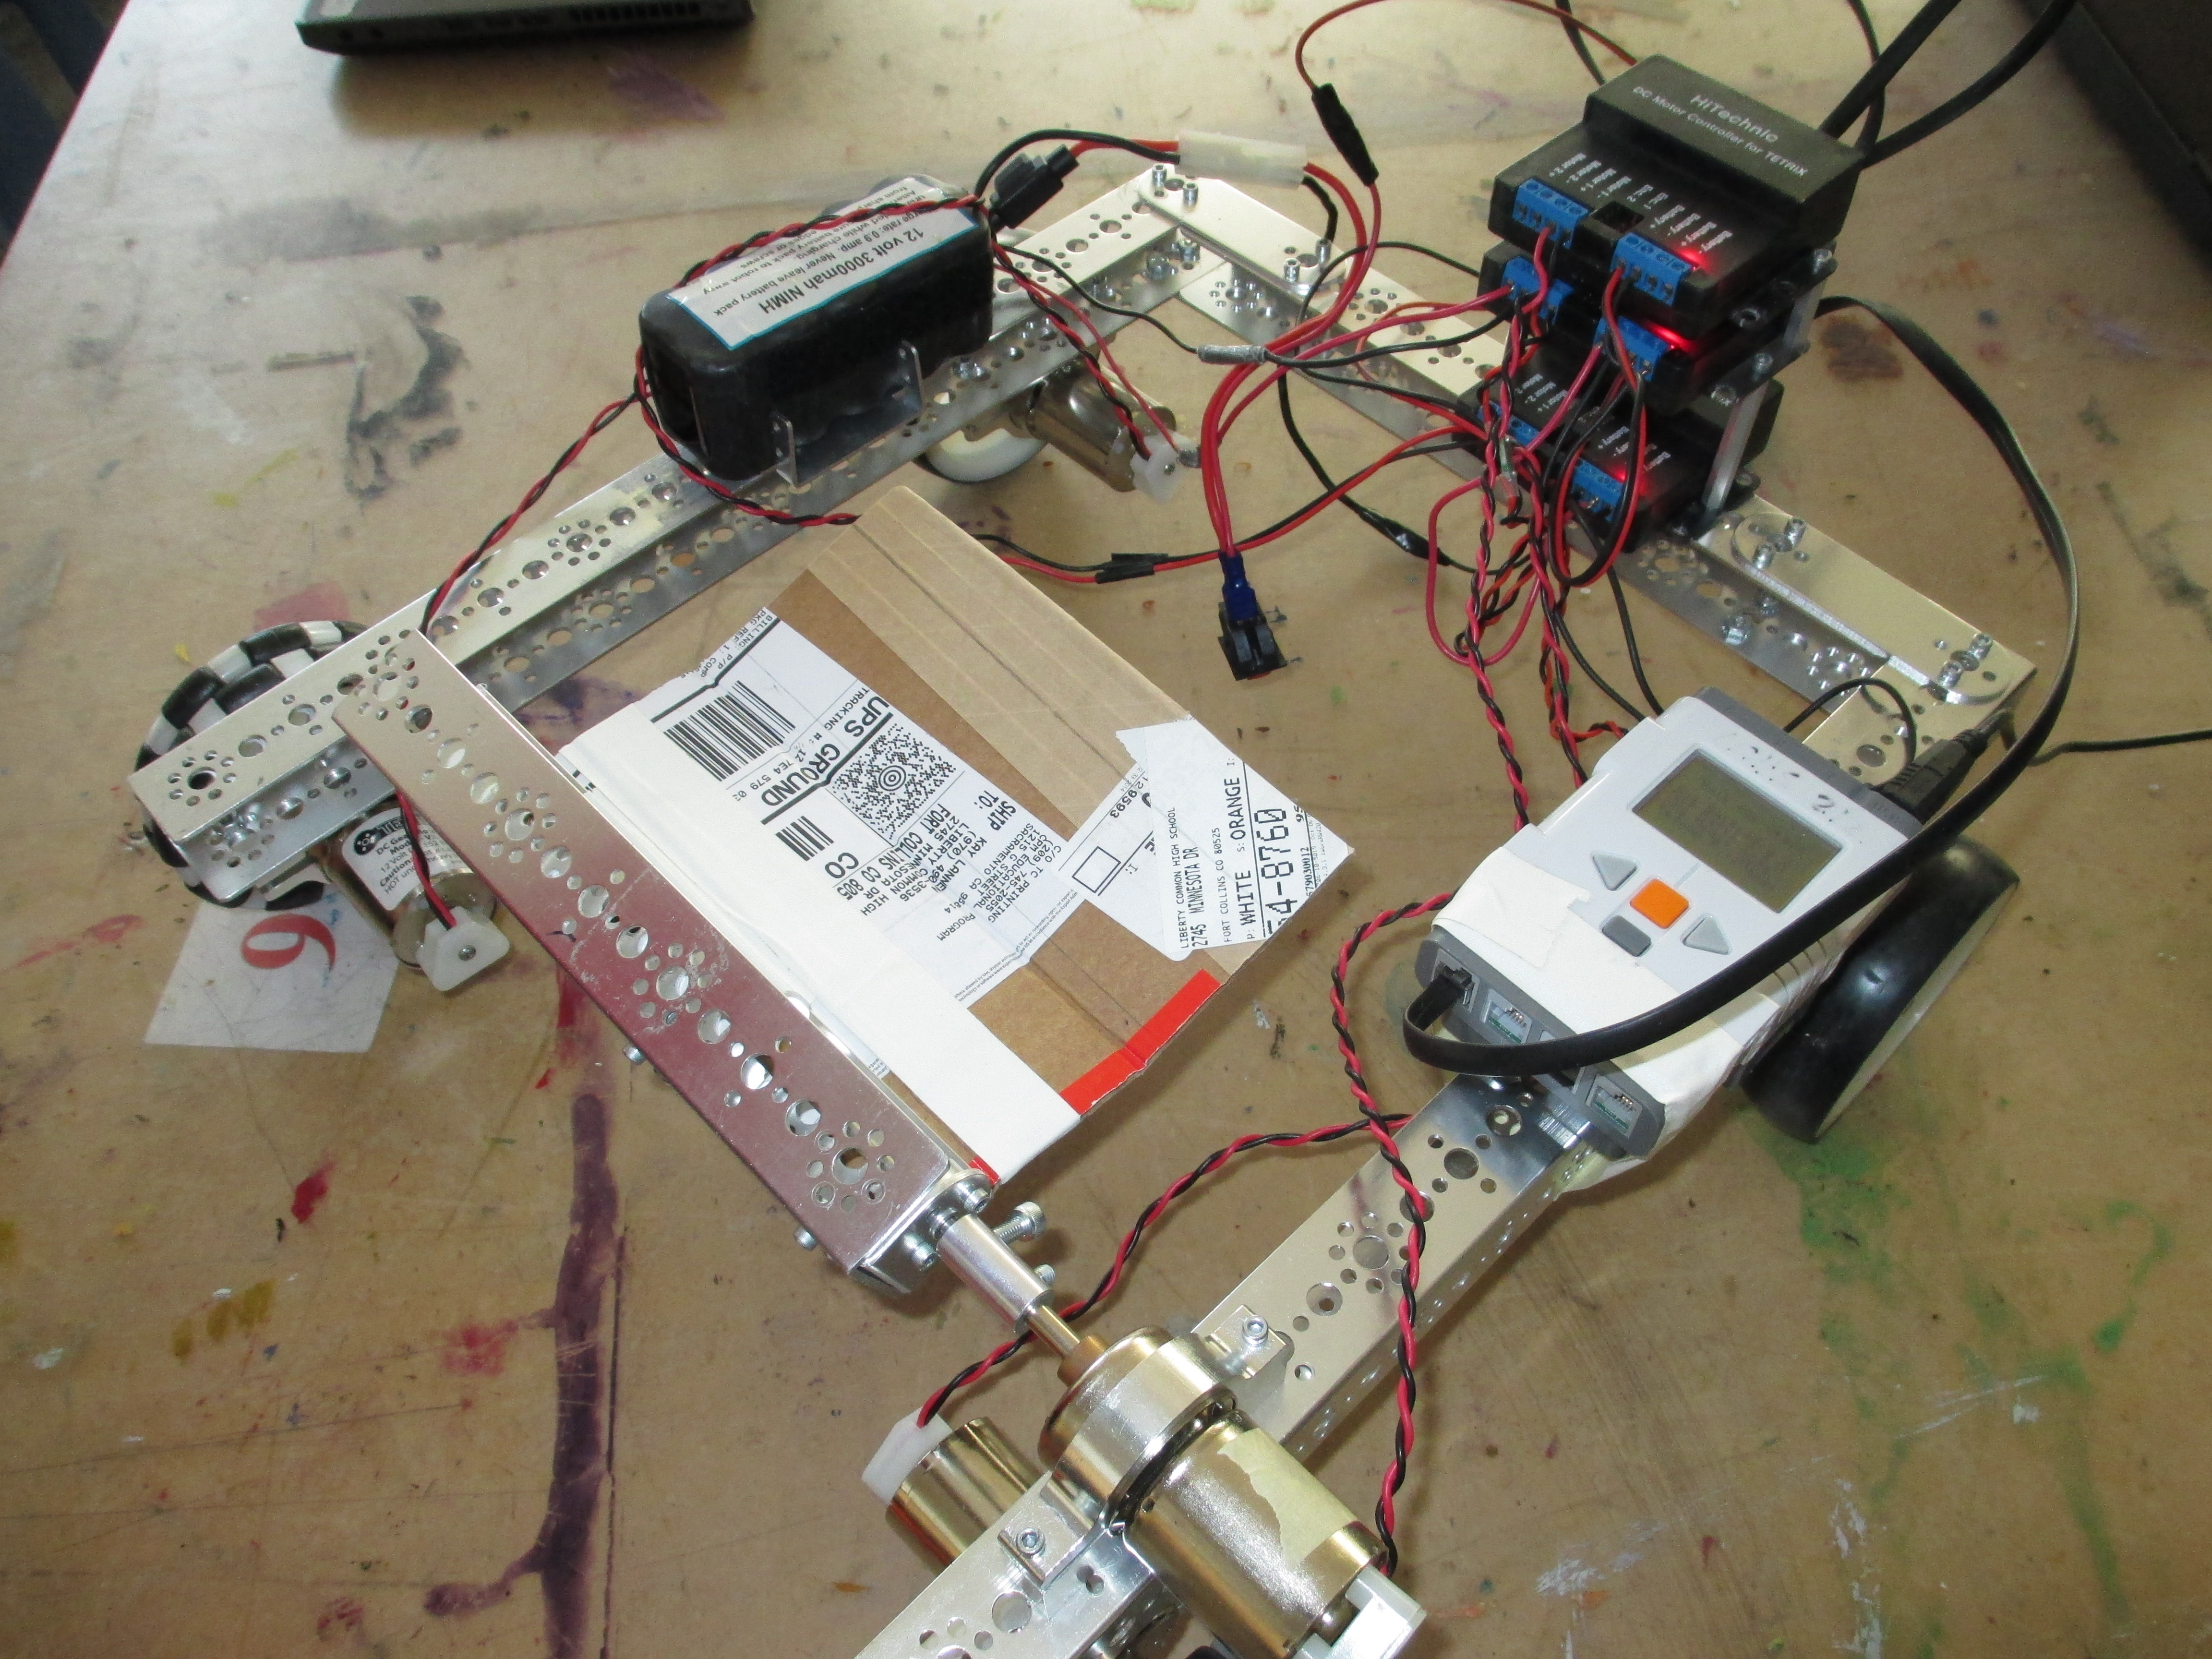
\includegraphics[width=10cm]{./Entries/Images/FirstRotatingBrushProto.JPG}
\end{center}

The first prototype of our rotating brush in the front of the robot. 